\documentclass{article}

\usepackage[utf8]{inputenc}
\usepackage{ngerman}
\usepackage{lmodern}
\usepackage{amsthm}
\usepackage{amssymb}
\usepackage{mathtools}
\usepackage{paralist}
\usepackage[paper=a4paper,left=25mm,right=25mm,top=25mm]{geometry}

\newtheorem{satz}{Satz}
\newtheorem{definition}[satz]{Definition}
\newtheorem{lemma}[satz]{Lemma}
\newtheorem{proposition}[satz]{Proposition}
\newtheorem{beweis}{Beweis}
%Create a new theorem by writing \newtheorem{How to call this type of theorem}[satz]{What should be written}. Make sure to keep "satz" to ensure consecutive numeration.
% %  Variablen Definition...............
\newcommand*{\R}{k[X_{1},\ldots,X_{n}]}
\newcommand*{\indx}[2]{{#1}_{#2}}
\newcommand*{\potx}[2]{{#1}^{#2}}
\newcommand*{\N}{\mathbb{N}_0}
\newcommand*{\hf}[1]{$\prescript{a}{}{HF}_{#1}$}
\newcommand*{\hp}[1]{$\prescript{a}{}{HP}_{#1}$}
\newcommand*{\kette}[2]{$1\leq {#1}_1<{#1}_2<{#1}_3<...<{#1}_{#2}\leq n$}
\newcommand*{\dkette}[2]{${#1}_1,{#1}_2,{#1}_3,\ldots,{#1}_{#2} \in \mathbb{N}$}
\newcommand*{\Rr}[2]{$ k[X_{{#1}_{1}},\ldots,X_{{#1}_{#2}}]$}
%\newcommand*{\hf}{}
\newcommand*{\ideal}{$I$}


\title{Dimension von Varietäten}
\date{\today}
\author{Yvan Ngumeteh \and Emma Ahrens}


\begin{document}

	\maketitle

	\begin{lemma} \label{1.2.3}
	Sei \(I \subseteq \R\) ein Ideal, das von einer Menge G von Monomen erzeugt wird. Dann liegt
	ein Polynom \(f \in \R\) in I genau dann, wenn für jeden Term \(a_{j}X^{\alpha_{j}}\) von f ein
	\(g \in G\) existiert, welches \(a_{j}X^{\alpha_{j}}\) teilt.
	\end{lemma}

	\begin{lemma} \label{1.2.4}
	Sei \((g_{i})_{i \geq 1}\) eine Folge von Monomen in \(\R\) mit \(g_{1} \succeq g_{2} \succeq
	\ldots\) für eine Monomialordnung \(\preceq\). Dann existiert ein \(r \in \mathbb{N}\) mit 
	\(g_{n} = g_{r}\) für alle \(n \geq r\). 
	\end{lemma}

	\begin{proposition}[Divisionsalgorithmus] \label{1.2.5}
	Sei \(\preceq\) eine Monomialordnung und \(f, f_{1}, \ldots, f_{s} \in \R\) nicht null. Dann
	gilt \begin{displaymath} f = \sum_{i=1}^{s} h_{i}f_{i}\; + r, \end{displaymath} mit
	\(r, h_{1}, \ldots, h_{s} \in \R\) und \(LT(h_{i}f_{i} \preceq LT(f)\) für alle \(h_{i} \neq 0
	\) und \(r = 0\) oder kein Term von r wird durch ein \(LT(f_{i})\) geteilt für \(i \in
	\underline{s}\).
	\end{proposition}

	\begin{satz} \label{1.2.8}
	Sei \(\{0\} \neq I \subseteq \R\) ein Ideal und \(\preceq\) eine Monomialordnung auf
	\(\mathbb{N}^{n}_{0}\). Sei G eine Gröbnerbasis von I mit I = (G). Dann ist eine k-Basis von 
	\(\R/I\) gegeben durch die Restklassen von \(X^{\alpha}\) mit
	\begin{displaymath}
	\alpha \in C(I) := \{\alpha \in \mathbb{N}^{n}_{0}\; |\;\; LT(g) \nmid X^{\alpha}\; \forall g 
	\in G\}.
	\end{displaymath}
	\end{satz}

	\begin{figure}[ht]
		\centering
		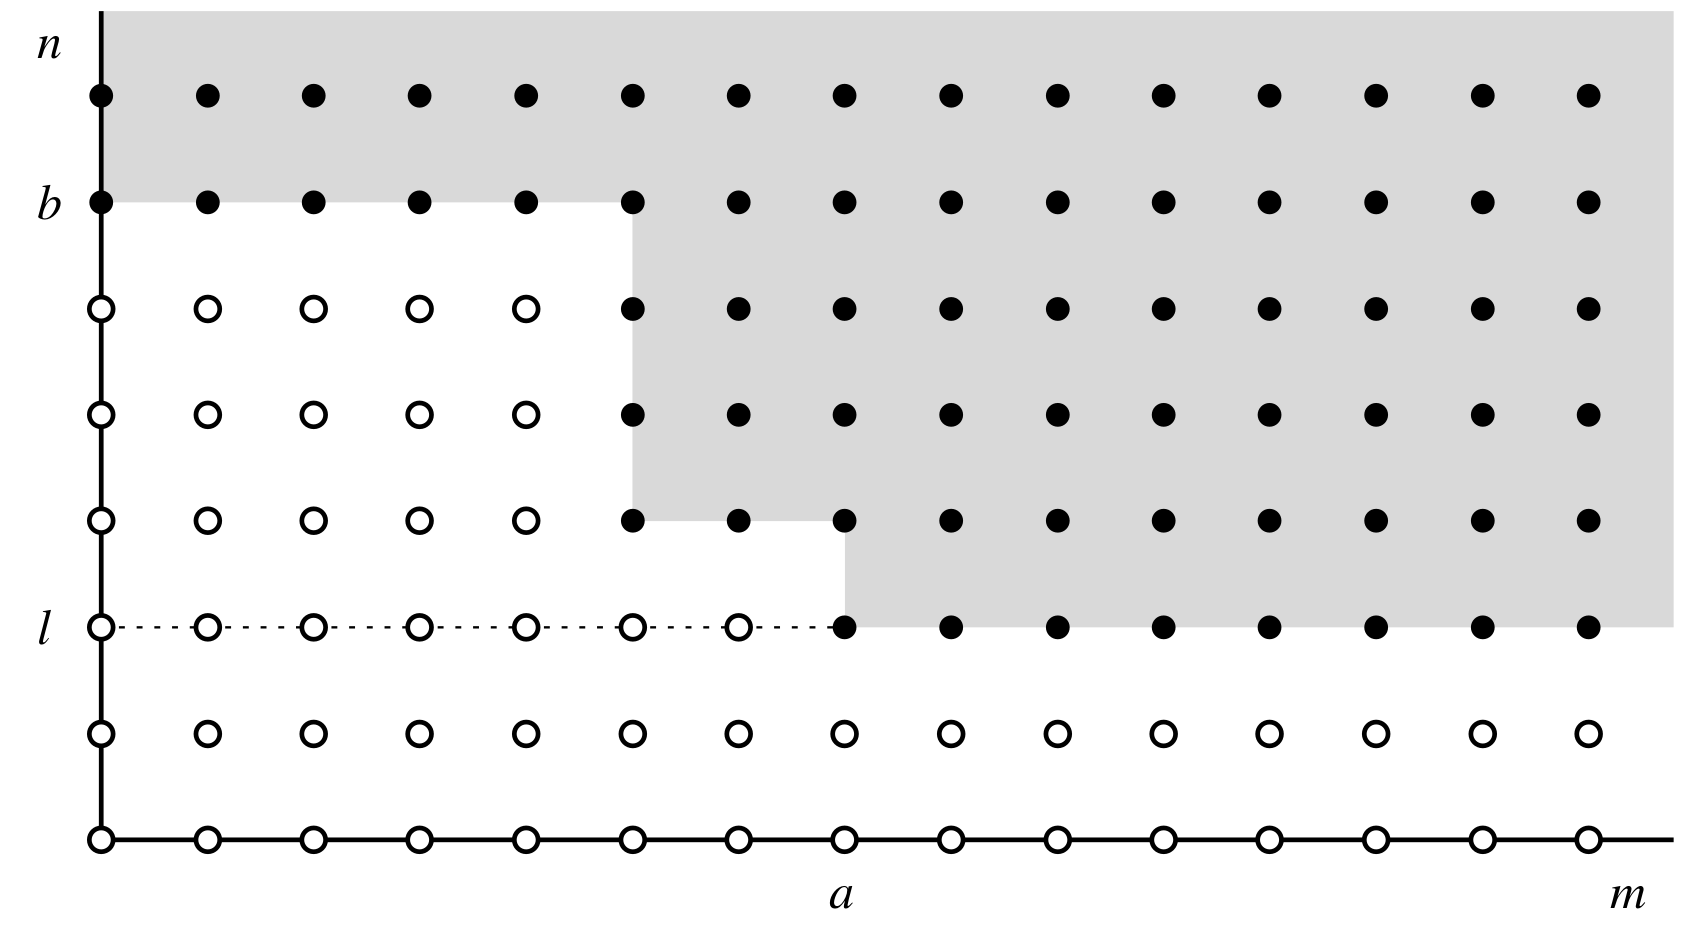
\includegraphics[width=.75\linewidth]{Dots.png}
		\caption{Anschauliche Darstellung von \(\R/I\) aus \cite{CLOS}}
		\label{dots}
	\end{figure}

	\begin{definition} \label{1.2.11}
	Sei \(I \subseteq \R\) ein Ideal und \(s \in \mathbb{N}_{0}\). Dann definiere \(I_{\leq s} :=
	I \cap \R_{\leq s}\). Nun gilt, dass \(\R_{\leq s}\) ein endlich dimensionaler Vektorraum über
	k  mit \(I_{\leq s}\) als Teilraum ist. Wir können die Funktion \begin{displaymath}
	\prescript{a}{}{HF}_{I} : \mathbb{N}_{0} \rightarrow \mathbb{N}_{0}, \quad s \mapsto
	dim_{k}(\R_{\leq s}/I_{\leq s})	\end{displaymath} definieren, die (affine) Hilbertfunktion
	von I genannt wird.
	\end{definition}

	\begin{lemma}
	Es gilt \(|M_{n,s}| := |\{\alpha \in \mathbb{N}^{n}_{0}\; |\; |\alpha| \leq s \}| = \binom{s + n}{s}. \)
	\end{lemma}

	\begin{lemma}[Macaulay] \label{1.2.13}
	Sei \(\preceq\) eine gradierte lexikographische Monomialordnung und \(I \subseteq \R\) ein
	Ideal. Dann ist \(\prescript{a}{}{HF}_{I}(s) = \prescript{a}{}{HF}_{LT(I)}(s)\) für alle
	\(s \in \mathbb{N}_{0}\).
	\end{lemma}


Im folgenden sei $n \in \mathrm{N}$ beliebig aber fest.

\begin{definition}[Buchberger]
	Sei $I\subset \R$ ein nicht triviales Ideal und $\preceq$ eine Monomiale Ordnung auf $\potx{\N}{n}$. Man nennt eine endliche Menge $G\subseteq I-\{0\}$ eine Gröbner-Basis von $I$, falls die Monome $LT(g)$ $(g\in G)$ das Ideal 
	\begin{displaymath}
	(LT(I)):=(LT(f):0\neq f\in I)\subseteq \R
	\end{displaymath}
	erzeugen. 
\end{definition}

Nach dem Hilbert'sche Basissatz besitzt jedes nicht triviales Ideal eine Gröbner-Basis.\\

\begin{satz}
	\label{1.2.14}
	Sei  \ideal $\unlhd$ $\R$, dann existiert ein eindeutiges Polynom \hp{I}(t) $\in \mathbb{Q}[t]$ (t ist eine Variable) und $\indx{s}{0}\geq0$,  sodass \hp{I}(s)=\hf{I}(s)= $\indx{dim}{k}$ ($\indx{\R}{\leq s}$/$\indx{I}{\leq s}$), für alle $ s\geq\indx{s}{0}$. Weiterhin besitzt \hp{I}(t) folgende Eigenschaften:	
\end{satz}v
\begin{compactenum}
	\item[a)] Der Grad von \hp{I}(t) ist der größte $d \in \mathbb{N}$, sodass es \dkette{i}{d} mit \kette{i}{d} existieren und $I\cap k[X_{{i}_{1}},\ldots,X_{{i}_{d}}]=(0)$.
	\item[b)] Sei $d=grad(\textnormal{\hp{I}})$. Dann gilt \hp{I}(t)=$\sum_{k=0}^{d} \indx{a}{k}t^k$ mit $\indx{a}{k}d! \in \mathbb{Z}, \forall k\in \underline{\indx{d}{0}}$ und $\indx{a}{d}d!>0$\\
\end{compactenum}

Sei $I\unlhd \R$ nicht trivial. Sei $G$ eine Gröbner-Basis von $I$ (bzgl. eine graduierte lexikographische Ordnung) und $M=\{\alpha \in \N^n:\exists\;f\in G \textnormal{ sodass } LM(f)=\potx{X}{\alpha}\}$
\begin{displaymath}
\{LM(g):g\in G\}=\{\potx{X}{\beta}:\beta \in M \}
\end{displaymath}

Die Mächtigkeit von $M$ ist endlich , da nach dem Hilbert'sche Basissatz $G$ eine endliche Menge von Polynomen ist.
Wir setzen im Folgenden 
\begin{displaymath}
C(I):=\{\alpha \in \N: \potx{X}{\beta} \nmid \potx{X}{\alpha},\; \forall \beta \in M \}
\textnormal{ und } 
\indx{C(I)}{\leq s}:= \{\alpha \in \N:|\alpha|\leq s \textnormal{ und } \; \potx{X}{\beta} \nmid \potx{X}{\alpha},\; \forall \beta \in M \}
\end{displaymath}

\begin{compactenum}
	\item Behauptung: $\forall s\geq 0$ gilt \hf{I}(s)$=|\indx{C(I)}{\leq s}|$.\\
	\item Seien $J\subseteq \underline{n}$ und eine Abbildung $\tau:J\longrightarrow \N$ gegeben. Wir definieren
	\begin{displaymath}
	C(J,\tau):=\{\alpha \in (\N)^n: \indx{\alpha}{j}=\tau(j), \forall \in J  \}
	\end{displaymath}
	
	Behauptung: Es existiert eine endliche Menge $\chi$ von Tupeln (J,$\tau$), sodass 
	
	\begin{displaymath}
	(\star)\;\;\;   C(I)=\bigcup\limits_{(J,\tau)\in \chi} C(J,\tau) =\bigcup\limits_{i\in \underline{l}} C(\indx{J}{i},\indx{\tau}{i})  
	\end{displaymath}
	wobei $l=|\chi|$ ist.\\
	\item Behauptung: Für alle $(J,\tau)$ im 2.Fall, existiert ein eindeutiges Polynom $\indx{F}{J,\tau}(s)\in \mathbb{Q}[t]$ mit $grad(\indx{F}{J,\tau})=n-|J|$ und
	$\indx{F}{J,\tau}(s)=\left|\indx{C(J,\tau)}{\leq s}\right|$, für alle $s\geq |\tau|:=\sum\limits_{j\in J}\tau(j)$\\
	\item Sei $m\in\N$ beliebig aber fest. Falls $\indx{A}{1},\ldots,\indx{A}{m}$ endliche Teilmengen von einer Menge $T$ sind, dann lässt sich die Mächtigkeit deren Vereinigung mittels dem Inklusion-Exklusion-Prinzip durch
	
	\begin{displaymath}
	\left|\indx{A}{1}\cup\ldots\cup\indx{A}{m}\right|=\sum\limits_{r=1}^{m}(-1)^{r-1}\sum\limits_{J\subset\underline{n},\left|J\right|=r}{|\bigcap\limits_{j\in J}\indx{A}{j}|}
	\end{displaymath}
	berechnen. Zusammen mit $(\star)$ und 3.Fall folgt für $s\geq \indx{s}{0}:=\max{\{\sum\limits_{i\in J\subset \underline{l}}|\indx{\tau}{i}|: J\subset \underline{l}\}}+1$ sowohl die eindeutige Existenz von \hp{I} als Polynom als auch die Aussage in $b)$. \\
	\item In diesem letzten Unterpunkt beweisen wir die Aussage in $a)$. Aus dem 4.Fall gilt, dass $grad(\textnormal{\hp{I}})$ die größte natürliche Zahl $d$ ist, sodass es ein $J\subset\underline{n}$ von $|J|=n-d$ und $\tau: J\rightarrow\N$ mit $C(J,\tau)\subset C(I)$  existiert. 
	
	Dies auch äquivalent mit der Aussage, dass $grad(\textnormal{\hp{I}})$ gegeben ist, durch $n-m$, wobei $m\in\mathbb{N}$ die minimale Anzahl von Variablen $\indx{X}{\indx{i}{1}},\ldots,\indx{X}{\indx{i}{m}}$ bezeichnet, sodass $\alpha=(0,\ldots,\indx{\alpha}{\indx{i}{1}}=1,0,\ldots,0,\indx{\alpha}{\indx{i}{m}}=1,0,0)\in C(I)$ gilt.\\
	
	Behauptung: Es gilt: $I\cap k\left[\indx{X}{j}:j\notin J\right]={(0)}$, für alle Tupel $(J,\tau)$ sodass $C(J,\tau)\subset C(I)$.\\
	
	Hieraus folgt, dass
	\begin{align*}
	grad(\textnormal{\hp{I}}(t))&\leq \max{\{d\in\underline{n}:\exists J\subset\underline{n}\, mit\,I\cap K[\indx{X}{j}:j\in J]=(0)\}}\\&
	= \max{\{d\in\underline{n}:\exists \indx{i}{1},\ldots,\indx{i}{n}\underline{n}\; \textnormal{ mit }  1\leq\indx{i}{1}<\ldots<\indx{i}{n}\leq n\;\textnormal{ und }I\cap K[\indx{X}{j}:j\notin J]=(0)\}}.
	\end{align*}
\end{compactenum}

% %
\begin{definition}
	Sei $V\subset k^n$ eine algebraische Menge und \hp{I(V)}(t) ist das Hilbert-Polynom von $I(V)\unlhd\R$ (nach Satz \ref{1.2.14} ist wohldefiniert und eindeutig). Für $V\neq\emptyset$ (d.h. $I(V)\neq\R$), wird die Dimension definiert als 
	
	\begin{displaymath}
	dim(V)=grad(\textnormal{\hp{I(V)}}).
	\end{displaymath}
	Eine etwas handlichere Charakterisierung ist nach Satz \ref{1.2.14} durch:
	
	\begin{displaymath}
	dim(I(V))=\max{\{d\in\underline{n}:\exists{\,} 1\leq\indx{i}{1}<\ldots<\indx{i}{d}\leq n \textnormal{ mit } I\cap K[\indx{X}{\indx{i}{1}},\ldots,\indx{X}{\indx{i}{d}}]=\{0\} \}}
	\end{displaymath}
	gegeben.\\
\end{definition}
Beispiel: 
\begin{compactenum}
	\item Für $V=\{v\}\subset k^n$ gilt $dim(V)=0$.
	\item Für $V\subseteq k^n$ gilt $dim(V)=n$ genau, dann wenn $V=k^n$.
	\item Sei $V=\indx{H}{f}$ mit $f\neq\; const.$ eine Hyperfläche, dann gilt $dim(V)=n-1$.\\
\end{compactenum}
% %

\begin{proposition}
	Sei $V\subseteq k^n$ algebraisch und $V=\bigcup\limits_{i\in\underline{r}}\indx{V}{i}$ eine Zerlegung in irreduziblen Komponenten (vgl. Proposition 1.1.11). Dann gilt
	\begin{displaymath}
	dim(V)=\max{\{dim(\indx{V}{i}):i\in\underline{r}\}}\\
	\end{displaymath}
	\\
\end{proposition}
Beispiel:
Der Hilbert'sche Nullstellensatz für Hyperfläche besagt: Zu $const.\neq f\in \R$ und $\indx{H}{f}\in k^n$, sodass $f=\prod\limits_{i=1}^{r} \indx{f}{i}$, wobei $\indx{f}{1},\ldots,\indx{f}{r}$ irreduzibel und paarweise teilerfremd sind, gilt
\begin{displaymath}
\indx{H}{f}=\bigcup\limits_{i=1}^{r} \indx{H}{f}\;\; \textnormal{und}\;\;I(\indx{H}{f})=(\indx{f}{1},\ldots,\indx{f}{r}).
\end{displaymath}

Die letzte Proposition liefert, dass es ein $i\in \underline{r}$ mit $dim(V)=dim(\indx{V}{i})$ gibt.\\ 
% %

Im Folgenden wollen wir eine andere Charakterisierung von $dim(V)$ angeben. 
\begin{definition}
	Sei $A$ eine $k-$Algebra (kommutativer, assoziativer $k-$Algebra mit 1). Man nennt $\indx{a}{1},\ldots,\indx{a}{m}\in A$ algebraisch unabhängig, falls 
	\begin{displaymath}
	\forall \;F\in k[\indx{X}{1},\ldots,\indx{X}{m}]\setminus\{0\} \;\textnormal{gilt}\; F(\indx{a}{1},\ldots,\indx{a}{m})\neq0.
	\end{displaymath}
	Man definiert
	\begin{displaymath}
	\indx{\partial}{k}(A):=\sup{\{m\geq0:\;\exists\; m \;\textnormal{algebraisch unabhängige Elemente in}\; A\}}
	\end{displaymath}
	Bemerkung: Falls A ein Körper ist, dann nennt man $\indx{\partial}{k}(A)$ der transcendenz Grad von $A$ über $k$.\\
\end{definition}

\begin{proposition}
	Sei $A:=\R/I$ mit $I\unlhd\R$ ein echtes Ideal. Dann gilt $grad(\textnormal{\hp{I}})=\indx{\partial}{k}(A)$. Ist $A$ weiterhin einen Integrietätsbereich $(IB)$ und $K$ ist der Quotienten-Körper von $A$, dann gilt
	\begin{displaymath}
	grad(\textnormal{\hp{I}})=\indx{\partial}{k}(A)=\indx{\partial}{k}(K).
	\end{displaymath}
	Insbesondere gilt $dim(V)=\indx{\partial}{k}(A[V])$ für jede nicht-leere algebraische $V\subset k^n$.\\
\end{proposition}

Beispiel: Aus dem 1.Vortrag gilt für den sog. \textquotedblleft Twisted Cubic\textquotedblright \;      $C=V((\indx{X}{2}-\indx{X}{1}^2,\indx{X}{3}-\indx{X}{1}^3))\subset k^n$, dass $I(C)=(\indx{X}{2}-\indx{X}{1}^2,\indx{X}{3}-\indx{X}{1}^3)$ und $\R/I(C)\cong k[Y]$. Wir zeigen
\begin{displaymath}
dim(C)=\indx{\partial}{k}(\R/I(C))=\indx{\partial}{k}(k[Y])=1.\\
\end{displaymath} 
\\

\begin{lemma}
	Sei $V\subseteq k^n$ irreduzible algebraischer Menge und $W\subseteq V$ abgeschlossenen Teilmenge. Dann gilt $dim(W)<dim(V)$, falls $W$ echte Teilmenge von $V$ ist.
\end{lemma} 


\begin{thebibliography}{99}
	\bibitem{CLOS}
	\textsc{Cox}, David; \textsc{Little}, John; \textsc{O'Shea}, Donal:
	\newblock \emph{Ideals, Varieties, and Algorithms}.
	\newblock Third Edition
	\newblock Springer-Verlag, 2007
\end{thebibliography}

\end{document}
